% !TEX root = ../document.tex
% !TeX spellcheck = pt_BR

\section{Método de Mohebbi e Moghadam}
\label{sec:section3}
Este método tem como principal recurso a obtenção de um modelo de batida cardíaca considerada normal, e extraída do próprio registro sobre o qual se deseja fazer a detecção de isquemia. As etapas do algoritmo podem ser visualizadas no diagrama da figura \ref{fig:mohebbi_01}, e sua implementação é descrita a seguir.

\begin{figure}[ht]
    \centering
    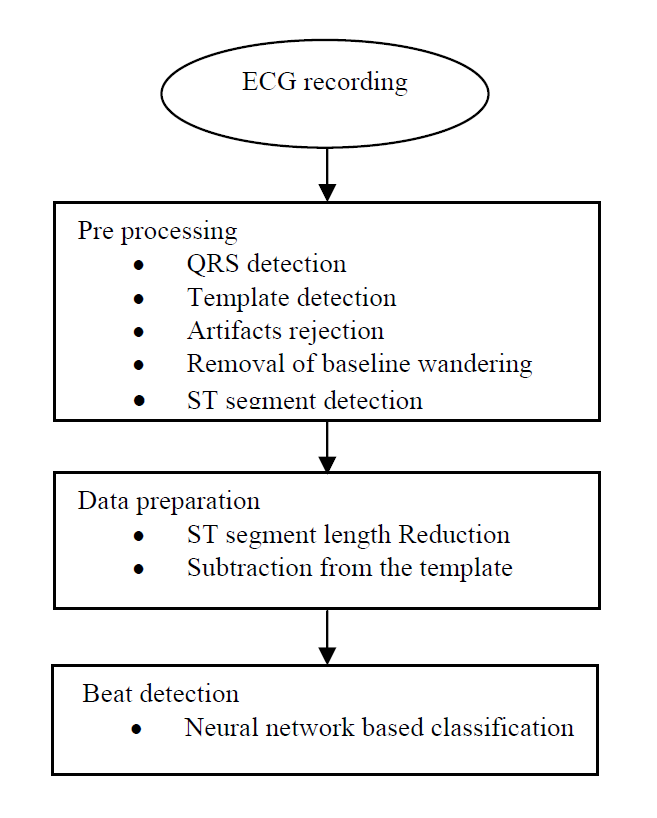
\includegraphics[width=0.6\textwidth]{figures/mohebbi_01.png}
    \caption{Diagrama de blocos da estratégia utilizada no método de Mohebbi e Moghadam. Extraído de \cite{Mohebbi07}}
    \label{fig:mohebbi_01}
\end{figure}

\subsection{Pré-processamento}
Esta etapa consiste de identificação dos complexos QRS, obtenção de um modelo, remoção de ruído, rejeição de artefatos e extração de segmento ST. A identificação dos complexos QRS, e respectivos picos, é feita através de um algoritmo descrito em \cite{Tompkins93}. Na saída obtêm-se uma lista com as localizações dos picos de onda R

Em seguida, os primeiros 30 segundos do registro de ECG são inspecionados afim de detectar artefatos (batidas anômalas). Este procedimento tenta detectar o nível isoelétrico e o ponto J de cada batida, através de uma análise do gradiente do sinal. Caso nenhum dos dois pontos seja detectado, a batida em questão é considerada como artefato, e removida da lista. As batidas remanescentes são usadas para construção do modelo, fazendo uma média das suas amplitudes.

Após este procedimento inicial, o resto do sinal é processado e a linha de base é estimada através de interpolação \emph{spline} cúbica, segundo o método proposto em \cite{Badilini91}. Uma vez removida a linha de base, detecta-se o ponto J de cada batida usando o mesmo procedimento mencionado no parágrafo anterior, usando o gradiente do sinal. Neste caso, uma janela de 100ms à direita do pico de onda R é suavizada por um filtro de média móvel e, em seguida, busca-se o primeiro intervalo de 20ms nesta janela cuja reta que melhor aproxima os pontos no intervalo possua um declive menor que 2,5$\mu$V/ms em valor absoluto. Toma-se o ponto que estabelece o início de tal intervalo como o ponto J.

Obtidos os pontos J, assume-se que os segmentos ST iniciem neste ponto e possuam tamanho pré-definido de 160ms. O mesmo vale para a batida modelo, de cujas amostras, usando o procedimento supracitado, extrai-se o segmento ST usado como referência. Chamar-lo-emos de $Y_{ST}$.

\subsection{Preparação dos dados}
Esta etapa é responsável por preparar os dados que servirão de entrada da rede neural. Dada uma taxa de amostragem $F_S$, o segmento ST possui $\lfloor0,16\cdot F_S\rfloor$ amostras. O conjunto de dados de entrada da rede neural é então obtido subtraindo-se as amplitudes de $Y_{ST}$ das do segmento ST de cada batida. Contudo, afim de reduzir o tamanho da entrada, os sinais que caracterizam os segmentos ST (inclusive o do modelo) são reamostrados fazendo a média entre duas amostras consecutivas, reduzindo assim pela metade o número de amostras. Em especial, no caso de uma taxa de amostragem $F_S = 250\mathrm{Hz}$, o segmento original conteria 40 amostras, enquanto o reamostrado contém apenas 20.

\subsection{Código MATLAB}
Um trecho de código da rotina principal do método é mostrado abaixo. Observe que a etapa de pré-processamento divide-se em duas partes: uma para processar os primeiros 30 segundos do ECG, contidos na variável \texttt{Signal1}; e outra para processar o resto do ECG, contido na variável \texttt{Signal2}.

\lstinputlisting[
    label=lst:mohebbi,
    caption={Trecho extraído do arquivo mohebbi.m}
]{listings/mohebbi.m}
